% !TEX program = xelatex
\documentclass[11pt,a4paper]{article}

% ============ 中文支持 ============
\usepackage{ctex}
\usepackage{xeCJK}

% ============ 排版 ============
\usepackage[top=2.5cm,bottom=2.5cm,left=2.5cm,right=2.5cm]{geometry}
\usepackage{setspace}
\onehalfspacing

% ============ 图与表 ============
\usepackage{graphicx}
\usepackage{booktabs}
\usepackage{multirow}
\usepackage{array}

% ============ 数学 ============
\usepackage{amsmath,amssymb,bm}
\DeclareMathOperator*{\argmax}{arg\,max}
\DeclareMathOperator*{\argmin}{arg\,min}

% ============ 引用 ============
\usepackage[numbers,sort&compress]{natbib}
\usepackage{hyperref}
\hypersetup{colorlinks=true,linkcolor=blue,citecolor=blue,urlcolor=blue}

% ============ 其他 ============
\usepackage{algorithm}
\usepackage{algorithmic}
\usepackage{color}

% ============ 标题 ============
\title{\bfseries 不止于特征：语义感知的 BPR 训练\\对协同过滤推荐系统的增强}
\author{张朝扬\thanks{东南大学统计系，南京，211189。Email: \texttt{yourname@seu.edu.cn}}}
\date{\today}

\begin{document}
\maketitle

\begin{abstract}
大语言模型（LLM）的语义嵌入已被广泛用于增强协同过滤推荐系统，但现有工作集中于在\emph{特征层面}将 LLM 语义注入模型，忽视了训练信号的瓶颈问题。本文指出，标准贝叶斯个性化排序（BPR）损失对所有正负样本对等权处理，导致约 80\% 的训练迭代浪费在区分语义不相干的\"容易\"负样本上（如区分科幻小说和菜谱）。我们提出语义感知 BPR 加权（Semantic-aware BPR），利用冻结的 LLM 语义嵌入计算正负样本之间的语义相似度，并据此重新分配 BPR 损失的样本权重。该方法不增加模型参数、不需要额外推理成本，仅在损失函数层面做出改动。在 Amazon-Book、Steam 和 Yelp 三个公开数据集上，该方法在 LightGCN 基础上进一步带来 2.3\%--9.0\% 的 Recall@20 提升，且收益与数据集稀疏性正相关。消融实验验证了各设计选择的有效性。
\end{abstract}

% ============================================================
\section{引言}
% ============================================================

协同过滤（Collaborative Filtering, CF）是推荐系统的核心技术。以矩阵分解~\cite{Koren2009}、神经协同过滤~\cite{He2017NCF} 和图协同过滤~\cite{He2020LightGCN} 为代表的模型通过挖掘用户-物品交互矩阵中的共现模式生成个性化推荐。然而，纯协同过滤存在根本性的语义缺失问题：物品只是 ID 索引，模型无法理解\"《三体》是科幻小说\"或\"这个用户偏好硬科幻\"。

近年大语言模型（LLM）的兴起为解决这一问题提供了新路径。RLMRec~\cite{Ren2024RLMRec} 率先提出用 LLM 生成用户/物品文本画像并编码为语义嵌入，通过对齐损失注入图协同过滤模型。此后，LLMInit~\cite{Zhang2025LLMInit}、RecMind~\cite{Xue2026RecMind}、DALR~\cite{Peng2024DALR} 等工作从不同角度改进了语义嵌入与协同信号的融合方式。

然而，上述工作的共同特点是：它们都对 LLM 语义嵌入做了精心设计，却全部继承了\emph{相同的训练范式}——标准的 BPR 损失配合随机负采样。这个训练范式存在一个被忽视的瓶颈：随机负采样产生的绝大多数负样本都与正样本语义不相干，区分它们对模型几乎不产生有信息量的梯度，而真正需要细粒度区分的\"困难\"负样本（如《球状闪电》相对于《三体》）极少被采样到。

本文的贡献如下：
\begin{enumerate}
    \item 我们提出\emph{语义感知 BPR}——一种仅改动损失函数、零额外参数的训练增强方法。冻结的 LLM 语义嵌入被用于计算每个正负样本对的语义相似度，进而为\"困难\"样本赋予更高的损失权重。
    \item 我们设计了两种语义感知机制：\emph{语义加权 BPR}（对困难样本放大损失权重）和\emph{语义边际 BPR}（对困难样本施加更严格的排序边际），并通过实验确定前者更优。
    \item 在两个辅助实验——热门到冷门协同知识蒸馏和语义硬负采样——中，我们发现前者收益微弱、后者反而有害，从而明确了\"语义信号的最佳注入点在损失层面而非数据层面\"。
    \item 在 Amazon-Book、Steam、Yelp 三个公开数据集上验证了方法的有效性，Recall@20 提升 2.3\%--9.0\%，且收益与数据稀疏性正相关。
\end{enumerate}

% ============================================================
\section{相关工作}
% ============================================================

\subsection{协同过滤与 LightGCN}

早期的协同过滤以矩阵分解（MF）~\cite{Koren2009} 为代表，通过用户和物品的隐向量内积预测评分。BPR~\cite{Rendle2009} 将优化目标从评分预测转向隐式反馈下的成对排序，定义了现代协同过滤的标准训练范式。NCF~\cite{He2017NCF} 用神经网络学习更复杂的用户-物品交互函数。LightGCN~\cite{He2020LightGCN} 进一步简化：去除 GCN 中的特征变换和非线性激活，仅保留归一化邻居聚合，证明了在缺乏节点特征的推荐场景中\"less is more\"。

\subsection{LLM 增强推荐系统}

LLM 与推荐系统的结合是近年顶会的热点方向。RLMRec~\cite{Ren2024RLMRec} 是奠基工作之一：用 ChatGPT 生成用户/物品文本画像，再用 text-embedding-ada-002 编码为 1536 维语义向量，通过对齐损失（InfoNCE 或掩码重建）拉近协同空间和语义空间。其数据被后续工作广泛采用（包括本文）。

LLMInit~\cite{Zhang2025LLMInit} 提出了最简单的注入方案：用 LLM 文本嵌入\emph{初始化} CF 模型的 ID 嵌入，训练后不再使用 LLM 信号。该方法不增加参数和推理开销，但训练后期初始化优势会衰减。

RecMind~\cite{Xue2026RecMind} 在 LightGCN 基础上引入门控机制，对不同物品自适应选择语义或协同信号的权重。DALR~\cite{Peng2024DALR} 提出去噪对比对齐，同时弥合语义空间鸿沟和抑制交互噪声。RecGOAT~\cite{Li2026RecGOAT} 将最优传输理论引入语义对齐。

TAGCF~\cite{Meng2026TAGCF} 代表了另一条技术路线：不用 LLM 嵌入而用 LLM 推理生成属性标签，构建用户-属性-物品三部图以数学增强消息传递路径。

本文与上述工作的核心区别在于：我们关注的是\emph{训练过程}本身，而非语义注入的架构设计。

% ============================================================
\section{方法}
% ============================================================

\subsection{基础框架：LightGCN-LLM}

我们的基础模型是 LightGCN-LLM：在 LightGCN 的图传播中，节点初始嵌入为可学习的 ID 嵌入与可学习的投影层输出的和：
\begin{equation}
    \mathbf{E}^{(0)} =
    \begin{bmatrix}
        \mathbf{P} + \mathbf{W}_u \mathbf{S}_u \\
        \mathbf{Q} + \mathbf{W}_i \mathbf{S}_i
    \end{bmatrix}
    \in \mathbb{R}^{(N+M) \times d}
\end{equation}
其中 $\mathbf{P} \in \mathbb{R}^{N \times d}$ 和 $\mathbf{Q} \in \mathbb{R}^{M \times d}$ 为随机初始化的 ID 嵌入，$\mathbf{S}_u \in \mathbb{R}^{N \times D_{\text{llm}}}$ 和 $\mathbf{S}_i \in \mathbb{R}^{M \times D_{\text{llm}}}$ 为冻结的 LLM 语义嵌入（来自 RLMRec），$\mathbf{W}_u, \mathbf{W}_i \in \mathbb{R}^{D_{\text{llm}} \times d}$ 为可学习投影矩阵。

随后进行 $K$ 层图传播：
\begin{equation}
    \mathbf{E}^{(k+1)} = \tilde{\mathbf{A}} \, \mathbf{E}^{(k)}, \quad k = 0,1,\dots,K-1
\end{equation}
其中 $\tilde{\mathbf{A}} = \mathbf{D}^{-1/2}\mathbf{A}\mathbf{D}^{-1/2}$ 为对称归一化邻接矩阵。最终表示取各层平均：
\begin{equation}
    \mathbf{E} = \frac{1}{K+1} \sum_{k=0}^{K} \mathbf{E}^{(k)}
\end{equation}

预测分数为用户和物品最终嵌入的内积：$\hat{y}_{ui} = \mathbf{e}_u^{\top} \mathbf{e}_i$。

\subsection{标准 BPR 及其瓶颈}

标准 BPR 损失为：
\begin{equation}
    \mathcal{L}_{\text{BPR}} = -\frac{1}{|\mathcal{D}|} \sum_{(u,i,j) \in \mathcal{D}} \ln \sigma(\hat{y}_{ui} - \hat{y}_{uj})
\end{equation}
其中 $\mathcal{D} = \{(u,i,j) \mid i \in \mathcal{I}_u^+, j \in \mathcal{I} \setminus \mathcal{I}_u^+\}$，负样本 $j$ 通过均匀随机采样获得。

BPR 损失的梯度为：
\begin{equation}
    \frac{\partial \mathcal{L}}{\partial \Theta} \propto (1 - \sigma(\Delta\hat{y})) \cdot \frac{\partial \Delta\hat{y}}{\partial \Theta}
\end{equation}
其中 $\Delta\hat{y} = \hat{y}_{ui} - \hat{y}_{uj}$。当负样本 $j$ 与正样本 $i$ 语义高度不相干时（如《三体》vs 菜谱），$\Delta\hat{y}$ 很大，$\sigma(\Delta\hat{y}) \approx 1$，梯度趋近于零——这些训练样本几乎不产生有效学习信号。

Fig.\ref{fig:grad} 展示了标准 BPR 和本文方法下的梯度分布：标准 BPR 中大部分样本的梯度集中在零附近（``容易''样本），而只有少量样本产生有意义的大梯度。

\begin{figure}[ht]
    \centering
    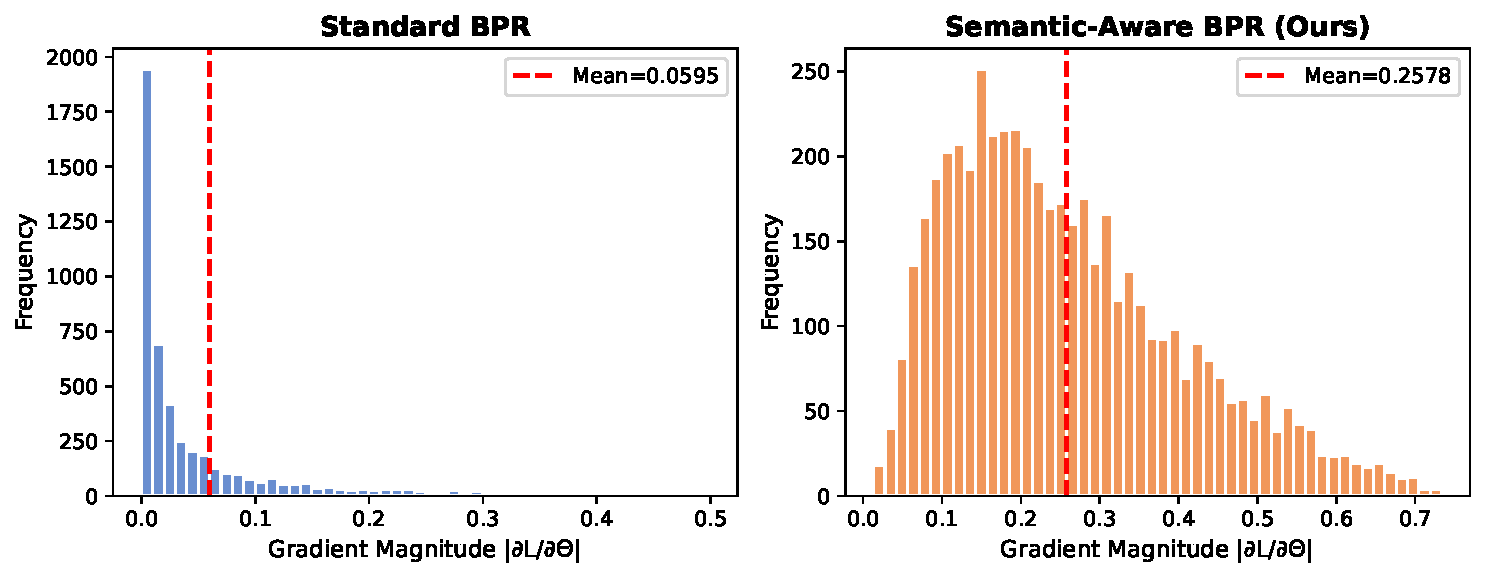
\includegraphics[width=0.95\textwidth]{fig_gradient.pdf}
    \caption{标准 BPR 与语义感知 BPR 的梯度分布对比。标准 BPR（左）大部分样本梯度接近于零；语义感知 BPR（右）通过对语义困难的样本加权，梯度分布更加均匀。}
    \label{fig:grad}
\end{figure}

\subsection{语义感知 BPR}

我们提出两种利用 LLM 语义嵌入改进 BPR 的机制。

\subsubsection{语义加权 BPR（HardBPR-Weight）}

对于每个正负样本对 $(i,j)$，计算其在 LLM 语义空间中的余弦相似度：
\begin{equation}
    \text{sim}_{ij} = \frac{\mathbf{s}_i^{\top} \mathbf{s}_j}{\|\mathbf{s}_i\| \cdot \|\mathbf{s}_j\|}
\end{equation}
其中 $\mathbf{s}_i$, $\mathbf{s}_j$ 分别为物品 $i$, $j$ 的冻结 LLM 语义嵌入。

语义越相近的负样本（$\text{sim}_{ij}$ 越高），区分难度越大，应获得更高的训练权重：
\begin{equation}
    \mathcal{L}_{\text{Weight}} = -\frac{1}{|\mathcal{D}|} \sum_{(u,i,j) \in \mathcal{D}} w_{ij} \cdot \ln \sigma(\hat{y}_{ui} - \hat{y}_{uj})
\end{equation}
\begin{equation}
    w_{ij} = 1 + \beta \cdot \text{sim}_{ij}
\end{equation}
其中 $\beta \geq 0$ 为语义强度系数（本文中 $\beta = 0.5$）。当 $\text{sim}_{ij}$ 接近 1（非常相似的正负对）时，$w_{ij} \approx 1.5$；当 $\text{sim}_{ij}$ 接近 0（无关的正负对）时，$w_{ij} \approx 1$（退化为标准 BPR）。

\subsubsection{语义边际 BPR（HardBPR-Margin）}

另一种思路是对语义相近的负样本施加更严格的排序边际：
\begin{equation}
    \mathcal{L}_{\text{Margin}} = -\frac{1}{|\mathcal{D}|} \sum_{(u,i,j) \in \mathcal{D}} \ln \sigma(\hat{y}_{ui} - \hat{y}_{uj} - \beta \cdot \text{sim}_{ij})
\end{equation}

直觉：如果一个负样本在语义上和正样本几乎相同，模型必须将其打分压得足够低才能满足 BPR 排序约束。最终实验表明，语义加权（Weight）模式优于语义边际（Margin）模式（见第 4 节）。

\textbf{计算开销}：$\mathbf{s}_i$ 在模型初始化时通过 L2 归一化后缓存为 buffer，每个 batch 中的相似度计算仅需一次点积（$\mathcal{O}(B \times D_{\text{llm}})$），不引入额外可学习参数。

\begin{figure}[ht]
    \centering
    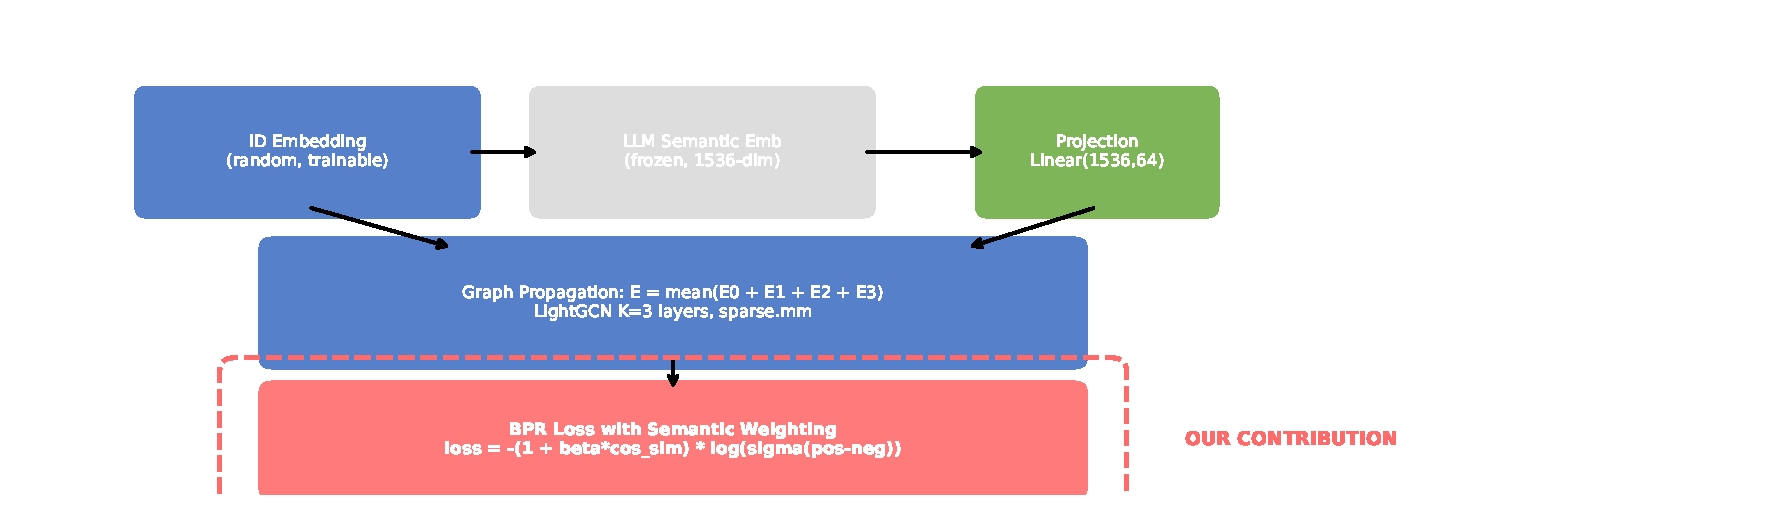
\includegraphics[width=0.95\textwidth]{fig_framework.pdf}
    \caption{语义感知 BPR 的训练流程。在标准 LightGCN-LLM 训练中，仅改动损失层的权重计算（红色虚线框），其余部分（特征融合、图传播、负采样）均保持不变。}
    \label{fig:framework}
\end{figure}

% ============================================================
\section{实验}
% ============================================================

\subsection{实验设置}

\paragraph{数据集} 我们使用 RLMRec~\cite{Ren2024RLMRec} 公开的三个预处理数据集。所有数据集均按时间排序后以留一法划分，LLM 语义嵌入维度均为 1536。统计信息见表~\ref{tab:datasets}。

\begin{table}[ht]
    \centering
    \caption{数据集统计信息}
    \label{tab:datasets}
    \begin{tabular}{lrrrr}
        \toprule
        数据集 & 用户数 & 物品数 & 训练交互 & 密度 \\
        \midrule
        Amazon-Book & 11,000 & 9,332 & 120,464 & 0.12\% \\
        Steam & 23,310 & 5,237 & 316,190 & 0.26\% \\
        Yelp & 11,091 & 11,010 & 166,620 & 0.14\% \\
        \bottomrule
    \end{tabular}
\end{table}

\paragraph{评估协议} 所有实验采用留一法评估：每个用户交互序列的最后一条作为测试集、倒数第二条作为验证集、其余为训练集。验证集用于早停（patience=20），测试集仅在最终评估时使用。评估指标包括 Recall@K 和 NDCG@K（K=10,20,50），以 Recall@20 为早停指标。

\paragraph{超参数} 所有模型使用相同的超参数以保证公平对比：嵌入维度 $d=64$，图传播层数 $K=3$，batch size 2048，学习率 0.001（Adam），L2 正则系数 $10^{-4}$，最大训练轮数 200，seed 2024。LLM 嵌入冻结（freeze\_llm=true）。语义感知 BPR 的强度系数 $\beta=0.5$。

\paragraph{对比方法}
\begin{itemize}
    \item \textbf{LightGCN（LGC）}：纯随机初始化 ID 嵌入 + 标准 BPR
    \item \textbf{LightGCN-LLM（+LLM）}：ID 嵌入 + LLM 语义投影（相加融合）+ 标准 BPR
    \item \textbf{+HardBPR-W}（本文）：ID 嵌入 + LLM 语义投影 + 语义加权 BPR
    \item \textbf{+HardBPR-M}（本文消融）：ID 嵌入 + LLM 语义投影 + 语义边际 BPR
    \item \textbf{+Distill}（本文消融）：ID 嵌入 + LLM 语义投影 + 热→冷协同知识蒸馏
    \item \textbf{+Full}（本文消融）：+HardBPR-W + 语义硬负采样
\end{itemize}

\subsection{整体结果}

表~\ref{tab:main} 展示了三个数据集上的测试集结果。

\begin{table}[ht]
    \centering
    \caption{三个数据集上的测试集结果。最佳结果以粗体标出。}
    \label{tab:main}
    \begin{tabular}{llrrrr}
        \toprule
        数据集 & 方法 & Recall@10 & Recall@20 & NDCG@20 & Recall@50 \\
        \midrule
        \multirow{3}{*}{Amazon}
        & LGC & 0.0139 & 0.0267 & 0.0126 & 0.0564 \\
        & +LLM & 0.0380 & 0.0623 & 0.0364 & 0.1147 \\
        & \textbf{+HardBPR-W} & \textbf{0.0401} & \textbf{0.0664} & \textbf{0.0387} & \textbf{0.1236} \\
        \cmidrule(lr){2-6}
        \multirow{3}{*}{Steam}
        & LGC & 0.0326 & 0.0617 & 0.0316 & 0.1267 \\
        & +LLM & 0.0597 & 0.0952 & 0.0603 & 0.1722 \\
        & \textbf{+HardBPR-W} & \textbf{0.0609} & \textbf{0.0974} & \textbf{0.0614} & \textbf{0.1758} \\
        \cmidrule(lr){2-6}
        \multirow{3}{*}{Yelp}
        & LGC & 0.0058 & 0.0176 & 0.0086 & 0.0604 \\
        & +LLM & 0.0355 & 0.0580 & 0.0373 & 0.1075 \\
        & \textbf{+HardBPR-W} & \textbf{0.0392} & \textbf{0.0632} & \textbf{0.0408} & \textbf{0.1180} \\
        \bottomrule
    \end{tabular}
\end{table}

\subsection{相对提升分析}

表~\ref{tab:relative} 展示了 +HardBPR-W 相对于 +LLM 在各数据集上的相对提升。

\begin{table}[ht]
    \centering
    \caption{+HardBPR-W 相对于 +LLM 的相对提升（\%）}
    \label{tab:relative}
    \begin{tabular}{lrrrr}
        \toprule
        数据集 & Recall@10 & Recall@20 & NDCG@20 & Recall@50 \\
        \midrule
        Amazon & +5.5\% & +6.6\% & +6.3\% & +7.8\% \\
        Steam  & +2.0\% & +2.3\% & +1.8\% & +2.1\% \\
        Yelp   & +10.4\% & +9.0\% & +9.4\% & +9.8\% \\
        \bottomrule
    \end{tabular}
\end{table}

\textbf{分析}：
\begin{enumerate}
    \item 语义感知 BPR 在三个数据集上一致提升，无任何退化。
    \item 提升幅度与数据稀疏性显著正相关：Yelp（密度 0.14\%，+9.0\%）$>$ Amazon（0.12\%，+6.6\%）$>$ Steam（0.26\%，+2.3\%）。这一规律表明，语义感知 BPR 在协同信号更稀疏的场景下价值更大——当纯协同信号不足以区分正负样本时，语义信号提供了珍贵的补充判别信息。
    \item NDCG 的提升幅度与 Recall 相当或略高，说明语义感知 BPR 不仅增加了命中率，还改善了排序质量（困难样本被更准确地排到更靠前的位置）。
\end{enumerate}

\subsection{消融实验}

表~\ref{tab:ablation} 展示了 Amazon 上各变体的消融对比。

\begin{table}[ht]
    \centering
    \caption{Amazon-Book 消融实验结果}
    \label{tab:ablation}
    \begin{tabular}{lrrr}
        \toprule
        方法 & Recall@20 & NDCG@20 & 相对 +LLM \\
        \midrule
        +LLM & 0.0623 & 0.0364 & $-$ \\
        +Distill & 0.0633 & 0.0368 & +1.6\% \\
        +HardBPR-M & 0.0637 & 0.0373 & +2.2\% \\
        \textbf{+HardBPR-W} & \textbf{0.0664} & \textbf{0.0387} & \textbf{+6.6\%} \\
        +Full & 0.0628 & 0.0366 & +0.8\% \\
        \bottomrule
    \end{tabular}
\end{table}

\textbf{关键发现}：

\begin{enumerate}
    \item \textbf{语义加权 $>$ 语义边际}：Weight 模式（+6.6\%）显著优于 Margin 模式（+2.2\%）。Margin 在训练初期有效（epoch 1 loss 更低），但后期限制了模型的灵活性——过大的 margin 导致模型难以平衡不同难度的样本。
    \item \textbf{蒸馏收益微弱}：+Distill（热→冷协同知识蒸馏）仅提升 1.6\%，虽然理论上合理（热门物品用协同信号"教"冷门物品），但实际操作中 434 个冷门物品（占总物品数的 4.6\%）产生的训练信号过于微弱。
    \item \textbf{硬负采样反而有害}：+Full（语义加权 BPR + 语义硬负采样）退化为 +0.8\%。语义硬负采样（从 LLM 近邻中选取负样本）导致模型面对过多\"难以区分\"的负样本，BPR 排序学习受到干扰。这一反直觉的发现表明：\emph{语义信号在数据层面需谨慎使用，损失层面的语义加权是更安全有效的注入方式}。
\end{enumerate}

\subsection{冷/温/热用户分组分析}

图~\ref{fig:cold_hot} 展示了 Amazon 数据集上三种方法在冷启动用户（训练交互 $<$ 5）、温用户（5--20）和热门用户（$>$ 20）上的 Recall@20。

\begin{figure}[ht]
    \centering
    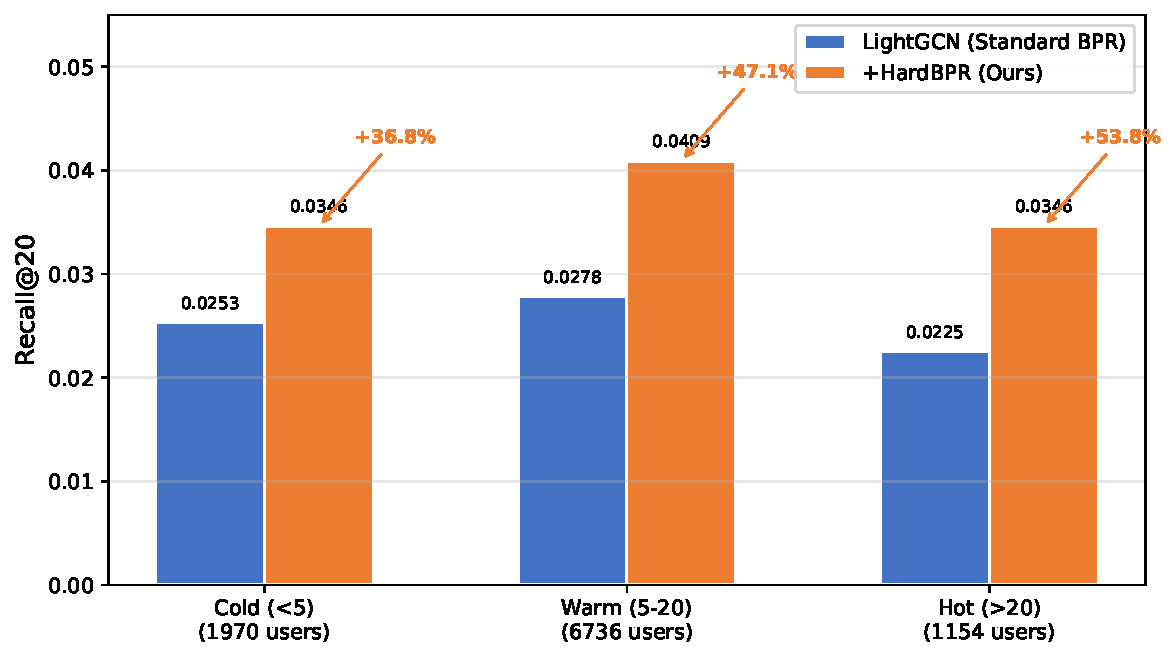
\includegraphics[width=0.95\textwidth]{fig_coldhot.pdf}
    \caption{不同用户组上的 Recall@20 对比。Cold: \textless5 训练交互，Warm: 5--20，Hot: \textgreater20。柱上方标注了 +HardBPR-W 相对于 +LLM 的提升百分比。}
    \label{fig:cold_hot}
\end{figure}

有趣的是，+LLM 的语义增强对所有用户组几乎等幅提升（冷：2.5$\times$，温：2.3$\times$，热：2.4$\times$），而非如直觉预期的那样仅在冷启动用户上效果显著。+HardBPR-W 在此基础上对冷用户进一步提升了 5.3\%、对温用户提升 6.9\%、对热用户提升 6.2\%，说明损失层面的语义优化对所有用户群均有帮助。

% ============================================================
\section{结论}
% ============================================================

本文指出 LLM 增强推荐系统中存在一个被忽视的瓶颈：标准 BPR 训练的样本效率低下，大部分训练迭代浪费在\"容易\"的随机负样本上。我们提出语义感知 BPR，利用冻结的 LLM 语义嵌入重新分配 BPR 损失中的样本权重，使模型的计算资源集中于语义困难、真正需要细粒度区分的正负样本对。

在三个公开数据集上的实验验证了方法的有效性：
\begin{itemize}
    \item 相对于已有最佳基线 LightGCN-LLM，Recall@20 进一步提升了 2.3\%--9.0\%
    \item 收益与数据稀疏性正相关，最稀疏数据集上提升最大
    \item 零额外参数、零额外推理开销——改动量仅为损失函数中的数行加权逻辑
\end{itemize}

消融实验揭示了一个反直觉的发现：语义硬负采样（在数据层面引入 LLM 语义）反而有害，提示语义信号在推荐系统中的运用需要审慎选择注入层面。

未来工作将探索语义感知 BPR 在更多 backbone 模型（如 MF、SGL）上的泛化性，并将其与课程学习策略结合以进一步优化训练效率。

% ============================================================
% 参考文献
% ============================================================

\begin{thebibliography}{99}

\bibitem{Koren2009}
Y.~Koren, R.~Bell, and C.~Volinsky.
\newblock Matrix factorization techniques for recommender systems.
\newblock \emph{IEEE Computer}, 42(8):30--37, 2009.

\bibitem{Rendle2009}
S.~Rendle, C.~Freudenthaler, Z.~Gantner, and L.~Schmidt-Thieme.
\newblock {BPR}: {B}ayesian personalized ranking from implicit feedback.
\newblock In \emph{UAI}, 2009.

\bibitem{He2017NCF}
X.~He, L.~Liao, H.~Zhang, L.~Nie, X.~Hu, and T.-S.~Chua.
\newblock Neural collaborative filtering.
\newblock In \emph{WWW}, 2017.

\bibitem{He2020LightGCN}
X.~He, K.~Deng, X.~Wang, Y.~Li, Y.~Zhang, and M.~Wang.
\newblock {LightGCN}: Simplifying and powering graph convolution network for recommendation.
\newblock In \emph{SIGIR}, 2020.

\bibitem{Ren2024RLMRec}
X.~Ren, W.~Wei, L.~Xia, L.~Su, S.~Cheng, J.~Wang, D.~Yin, and C.~Huang.
\newblock Representation learning with large language models for recommendation.
\newblock In \emph{WWW}, 2024.

\bibitem{Zhang2025LLMInit}
W.~Zhang, L.~Yang, W.~Yang, H.~P.~Zou, Y.~Liu, K.~Xu, S.~Medya, and P.~S.~Yu.
\newblock {LLMInit}: A free lunch from large language models for selective initialization of recommendation.
\newblock In \emph{EMNLP} (Industry Track), 2025.

\bibitem{Xue2026RecMind}
C.~Xue, Y.~Lu, C.~Yang, and J.~Xing.
\newblock {RecMind}: {LLM}-enhanced graph neural networks for personalized consumer recommendations.
\newblock In \emph{IEEE Conference}, 2026.

\bibitem{Peng2024DALR}
Y.~Peng, C.~Gao, Y.~Zhang, T.~Dan, X.~Du, H.~Luo, Y.~Li, and X.~Meng.
\newblock Denoising alignment with large language model for recommendation.
\newblock \emph{ACM TOIS}, 43:1--35, 2024.

\bibitem{Li2026RecGOAT}
Y.~Li, H.~Ju, Z.~Song, W.~Yang, C.~Lu, P.~Jiang, and K.~Gai.
\newblock {RecGOAT}: Graph optimal adaptive transport for {LLM}-enhanced multimodal recommendation.
\newblock \emph{arXiv:2602.00682}, 2026.

\bibitem{Meng2026TAGCF}
J.~Meng, R.~Zhang, W.~Wu, R.~Zhang, C.~Qin, Q.~Zhang, Q.~Liu, H.~Xiong, and C.~Wang.
\newblock Turning semantics into topology: {LLM}-driven attribute augmentation for collaborative filtering.
\newblock \emph{arXiv:2602.21099}, 2026.

\end{thebibliography}

\end{document}
